\part{Administración de memoria}
\section{Espacio de direcciones}
La parte del sistema operativo que maneja la jerarquía de memoria se llama \textbf{Memory Managment Unit (MMU)}. Su trabajo es mantener un registro de las partes de la memoria que están en uso, reservarla para los procesos que la necesitan y liberarla cuando ya no.

Uno de los métodos más simple de manejo memoria es permitir al programador usar la memoria física directamente.En este caso, se le presenta con un conjunto de direcciones que van desde 0 hasta algún máximo y el proceso ocupa toda la memoria disponible al momento de ejecutarse por lo que se debe esperar a que finalice antes de ejecutar otro.

En sistemas multi-usuarios, n tener varios procesos ejecutando de manera simultanea. Dado que esta situación es difícil de conseguir sin ningún tipo de abstracción, se agregó lo que se conoce como \textbf{espacio de memoria} de un proceso que es el conjunto de direcciones a las que tiene permitido acceder. 

Para separar los espacios de memoria entre distintos procesos, la implementación más simple consiste en agregar dos registros que indiquen cual es la primer dirección de memoria que tiene disponible (\textbf{base register}) y cual es el rango de memoria que puede usar (\textbf{limit register}). 

De esta forma, cuando el programador escribe su programa,  lo hace como si la dirección de memoria más baja disponible fuese la $0000000$. Cuando el proceso haga alguna referencia a memoria, el valor descrito por el programador es sumado al valor del registro base y se comprueba que la dirección resultante no supere el rango definido por el límite.

\subsection{Swapping}
Los métodos vistos hasta ahora permiten asignar a cada proceso un área de memoria. Si queremos ejecutar uno nuevo pero la misma está llena, debemos esperar a que uno o más procesos terminen hasta que se libere el espacio necesario para almacenar el nuevo proceso.

La técnica de \textbf{swapping} trata de resolver este problema guardando los estados de los procesos en ejecución en disco para luego poder cargar el estado de un nuevo proceso y ejecutarlo. Entonces, mientras haya espacio, se cargan y ejecutan como veníamos haciendo hasta ahora. Cuando se llena, se toma alguno de los procesos que se estén ejecutando, se guarda su estado en disco y se lo remplaza por el nuevo. A partir de aquí, cada proceso ejecuta por un tiempo determinado y luego se lo remplaza por otro que esté en la lista de espera.

En este caso no se asegura que los procesos sean cargados en el mismo área de memoria. Cada vez que se recarga uno, se deben reubicar las direcciones a las que hace referencia. 

Además, como no todos los procesos ocupan el mismo espacio en memoria, cuando se realiza un \textit{swap} pueden quedar bloques de memoria vacíos entre dos de ellos. Este efecto se llama \textbf{fragmentación externa} y es un problema porque tras varios swaps pueden quedar varios bloques pequeños vacíos dispersos por toda la memoria. Estos bloques son inutilizables pero si estuviesen todos aglomerados en algún sector específico podrían usarse para correr otro proceso por lo que estaríamos desperdiciando memoria.

Una forma de solucionar este problema es \textbf{compactar la memoria} cada vez que se realiza un swap. Esto es, mover todo los procesos cargados al principio de la memoria, dejando todo el espacio libre al final. Sin embargo, realizar esto cada vez que se realiza un intercambio es demasiado costoso por lo que no es una técnica utilizada.

Por otro lado, si el sistema operativo ofrece la posibilidad de reservar memoria de manera dinámica entonces el área de datos de un proceso debe tener la posibilidad de crecer:
\begin{itemize}
	\item Si la ubicación del mismo es adyacente a un bloque vacío entonces se puede agrandar su área de memoria sin problemas.
	\item Si no es adyante a ningún bloque, entonces el proceso se tiene que mover a un bloque lo suficientemente grande para alojarlo y, si este bloque no existe, se deberá swappear uno o más procesos para crear dicho bloque.
\end{itemize}

\subsection{Manejo de memoria libre}

Cuando la memoria es asignada de manera dinámica, el sistema operativo de mantener un registro preciso de que partes están ocupadas y cuales no. En general, para realizar esto, se puede utilizar alguna de las siguientes estructuras: un \textbf{bitmap} o una \textbf{lista enlazada}.

\begin{figure}[h]
	\centering
	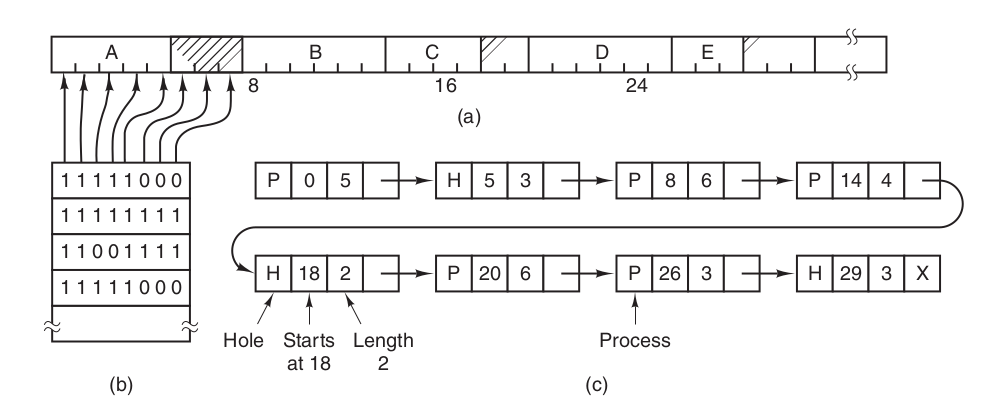
\includegraphics[width=0.65\textwidth
]{imagenes/bitmap-enlazada}
	\caption[Pedazo de memoria con cinco procesos y 3 bloques vacios.]{(a) Pedazo de memoria con cinco procesos y 3 bloques vacios. (b) Bitmap que representa el estado de la memoria. (c) Lista enlazada que representa el mismo estado.}
	\label{fig:bitmap-enlazada}
\end{figure}


\subsubsection{Bitmaps} 
La memoria se divide en bloques de igual tamaño llamados \textbf{unidades de reserva } a las que se les asigna un bit en un array que tiene tantos elementos como bloques haya. Si el bit correspondiente a una unidad se encuentra en cero (0) entonces está libre. Si es uno (1), la unidad está asignada a un proceso.

El tamaño de la unidad de reserva es una decisión de diseño. Mientras más chico sea, más unidades de reservas habrá pero el bitmap se hará más grande. En cambio, si se elige una tamaños demasiado grande, el bitmap se hará más pequeño pero podría desperdiciarse mucha memoria si los tamaños de los procesos no son múltiplos de ese tamaño (muchas unidades reservadas no serán usadas en su totalidad).

El principal problema que tiene esta estructura es que cuando se debe cargar un proceso de $k$ unidades de tamaño, el Memory Managment Unit debe buscar de manera lineal una secuencia de $k$ ceros consecutivos, lo que puede llegar a ser muy lento.

\subsubsection{Listas enlazadas} Otra forma de representar la memoria es mantener una lista enlazada de bloques reservados y espacios libres. Cada entrada de la lista especifica si el bloque pertenece a algún proceso o si está vacío, la dirección de memoria en la que empieza, su longitud y un puntero al próximo bloque. De esta forma es facil encontrar el bloque correspondiente a cada proceso (podemos agregar un puntero en el PCB que apunte al mismo) y liberar su memoria (y combinar bloques vacios) solo implica modificar un par de valores.

\begin{figure}[h]
	\centering
	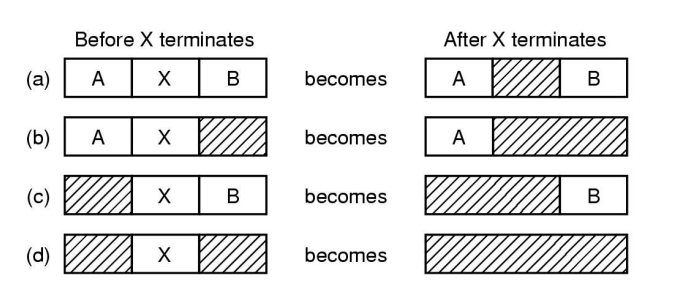
\includegraphics[width=0.7\textwidth]{imagenes/terminacion-proc-memoria}
	\caption{Cuatro combinaciones de vecinos para el proceso X}
	\label{fig:terminacion-proc-memoria}
\end{figure}

\subsubsection{Algortimos para reservar memoria}
Dado un proceso de tamaño $K$ debemos asignarle un espacio de la memoria para que pueda ser ejecutado. Sabemos que el área asignada tiene ser lo suficientemente grande como almacenarlo, el problema es decidir cuál de todos los espacios válidos elegimos. Para esto contamos con los siguientes algoritmos, entre otros:

\begin{itemize}
	\item \textbf{First Fit:} El MMU escanea la meoria hasta que encuentra un bloque lo suficientemente grande como para almacenar el proceso y ocupa la parte necesaria dejando la parte sobrante como un nuevo bloque vacío más pequeño.
	\item \textbf{Best Fit:} El MMU escanea toda la lista (de principio a fin) en busca de todos los bloques en los que podría caber el proceso. Luego le asigna el bloque más pequeño encontrado. En vez de partir un bloque grande, trata de que el bloque extra resultante sea lo más pequeño posible.
	
	Este algoritmo es un poco más lento que el anterior pero tampoco soluciona el problema de fragmentación.
	
	\item\textbf{Quick Fit:} Es una variación de los algoritmos anterior en la que se mantiene una lista de los bloques disponibles ordenado por tamaño. Aquí es facil encontrar un bloque adecuado pero cuando proceso termina o se swappea es más complejo combinar bloques vacíos.
\end{itemize}

\printbibliography[keyword=swapping,title=Bibliografía]

\newpage
\section{Memoria virtual}
Si bien los registros de base y límite nos permiten abstraernos un poco de la memoria, tienen sus limitaciones: Debemos cargar el proceso completo en memoria para poder ejecutarlo. Con los tamaños del softare de hoy en dia, surge la necesidad  de correr programas que no entran en memoria o que si bien entran de manera aislada cuando se lo corre en un sistema multi-usuario con otros procesos, no entran completamente en memoria.

El método diseñado para resolver el problema se conoce como \textbf{memoria virtual}. La idea es que cada proceso tiene definido un espacio de direcciones contiguo a los que puede hacer referencia. Cada una de estas direcciones está mapeada a una dirección física pero dos direcciones virtuales y deben ser traducidas para poder acceder a la información que se está solicitando.

\begin{figure}[h]
	\centering
	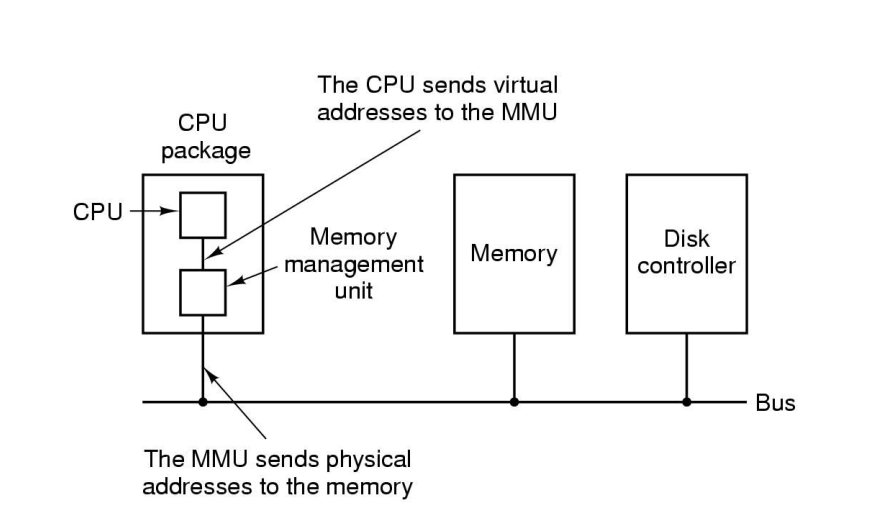
\includegraphics[width=0.7\textwidth]{imagenes/mmu-paging}
	\caption{Funcionamiento del Memory Managment Unit}
	\label{fig:mmu-paging}
\end{figure}

\subsection{Paginación}\label{paginacion}
La mayoría de los sistemas que usan memoria virtual implementan una técnica conocida como \textbf{paginación}: Cada programa tiene asignado un espacio de memoria virtual dividido en pedazos llamados \textbf{páginas}. Cada página es un rango continuo de direcciones y está mapeada a un pedazo de memoría física llamado \textbf{page frame}.

\begin{figure}[h]
	\centering
	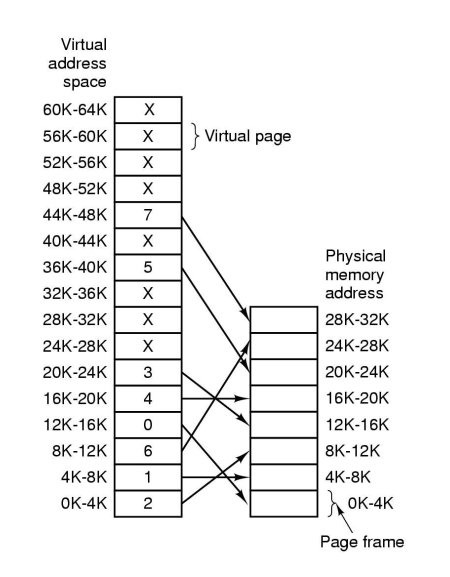
\includegraphics[width=0.6\textwidth]{imagenes/paging-mapping}
	\caption{Ejemplo de mapeo de direcciones virtuales a direcciones físicas}
	\label{fig:paging-mapping}
\end{figure}

Entonces un proceso puede comenzar a ejecutar sin necesidad que todas sus páginas estén cargados en memoria. Cuando hace referencia a una \textbf{dirección virtual}, la misma se envía al MMU que se fija si el page frame correspondiente está cargado en memoria. Si lo está entonces recupera la información pedida. Si no, emite un \textbf{page fault} que es atrapado por el sistema operativo que se encarga de traer el page frame necesario para poder continuar con la ejecución.

\subsubsection{Page tables} 
En esta implementación usamos una tabla para mapear direcciones virtuales a físicas. Dada una dirección virtual, la partimos en dos: 
\begin{itemize}
	\item \textbf{Número de página:} Son los bits más significativos. Nos indicara cuál es la posición de la tabla que apunta al page frame que contiene la dirección física deseada.
	\item \textbf{Offset:} Son los bits menos significativos. Se suman a la dirección del page frame encontrado  para poder conseguir la dirección de memoria física deseada.
\end{itemize}

\begin{figure}[h]
	\centering
	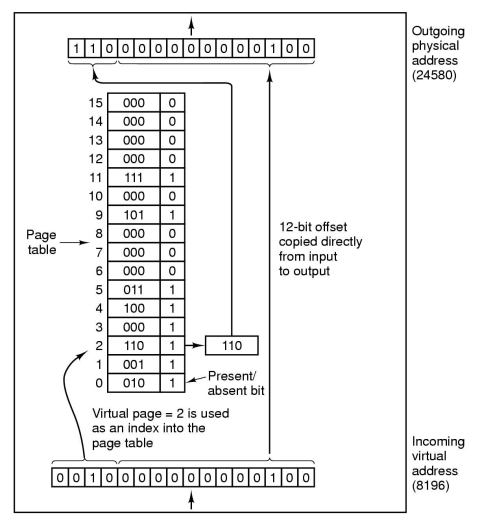
\includegraphics[width=0.5\textwidth]{imagenes/virtual-a-fisica}
	\caption[]{Conversión de una dirección virtual a una física}
	\label{fig:virtual-a-fisica}
\end{figure}

\subsubsection{Estructura de una entrada de la tabla de páginas}
Cada entrada de esta tabla tendrá la siguiente información, en la mayoría de los sistemas:

\begin{itemize}
	\item \textbf{Número de page frame:} El page frame al que mapea una página virtual.
	\item \textbf{Bit de presente/ausente:} Este bit es el que usa la MMU para saber si la entrada es válida (el page frame está cargado en memoria) o no.
	\item \textbf{Bit de protección:} Indica que tipo de accesos son permitidos. En su versión más simple, si está activo, el proceso solo puede leer. Si no lo está entonces puede escribir y leer.
	\item \textbf{Bit dirty:} Indica si la página fue modificada o no por el proceso. Este bit lo usa el sistema operativo cuando necesita desalojar el page frame. Si fue modificado, debe copiarse a disco sino la podemos sobrescribir ya que la copia en disco sigue siendo valida.
	\item \textbf{Bit de referencia:} Indica si la página fue referenciada por el proceso (tanto para escribir como para leer). Este bit tambien es usado por el sistema operativo para ayudarlo a decidir que page frame desalojar en caso de ser necesario. Las páginas que no están siendo usadas son mejores candidatos que aquellas que fueron referenciadas últimamente.
\end{itemize}

\subsection{Optimizaciones para paging}
Un sitema con paginación tiene que tener en cuenta dos cosas:
\begin{itemize}
	\item El mapeo de direcciones virtuales a físicas debe ser rápido.
	\item Si el espacio virtual es grande, entonces la tabla de páginas tambien lo será.
\end{itemize}
\subsubsection{Translation Lookaside Buffer (TLB)}
Para acelerar el mapeo de direcciones, se agregó al procesador una caché llamada \textbf{Translation Lookaside Buffer} o \textbf{Memoria asociativa} que permite realizar el mapeo sin tener que acceder a la tabla de páginas.

Cada entrada de esta cache contiene información sobre una página (su índice en la tabla de páginas, bit de protección, dirty y el page frame que le corresponde) además de un bit que indica si la entrada es válida.

Cuando la MMU recibe una dirección virtual, el hardware primero se fija si el número de página está presente en la TLB comparandolo simultáneamente con todas las entradas de la misma. Si lo encuetnra y el acceso no viola los bits de protección entonces el page frame se obtiene directamente. Si lo encuentra pero el proceso no tiene los permisos necesarios, entonces se genera un page fault.

Cuando ninguna de las entradas contiene el número de página buscado, el MMU detecta el \textit{miss} y realiza la búsqueda en la tabla de páginas de manera normal. Una vez encontrada, borra una de las entradas de la TLB y la remplaza con la entrada de la página encontrada.

Cuando una entrada se borra de la TLB, el bit de dirty se copia a la entrada de la page table correspondiente.

\subsubsection{Multilevel Page Tables}
El segundo problema que teniamos que resolver era como manejar tablas de páginas muy grandes. Esto se hace usando \textbf{tablas de página multinivel}. 

La idea es evitar que la tabla de páginas se mantenga completamente en memoria. En particular, aquellas entradas que no se necesitan no deberían mantenerse cargadas. Para conseguir esto, creamos un \textbf{directorio de páginas} y particionamos la tabla de páginas en partes iguales.

\begin{figure}[h]
	\centering
	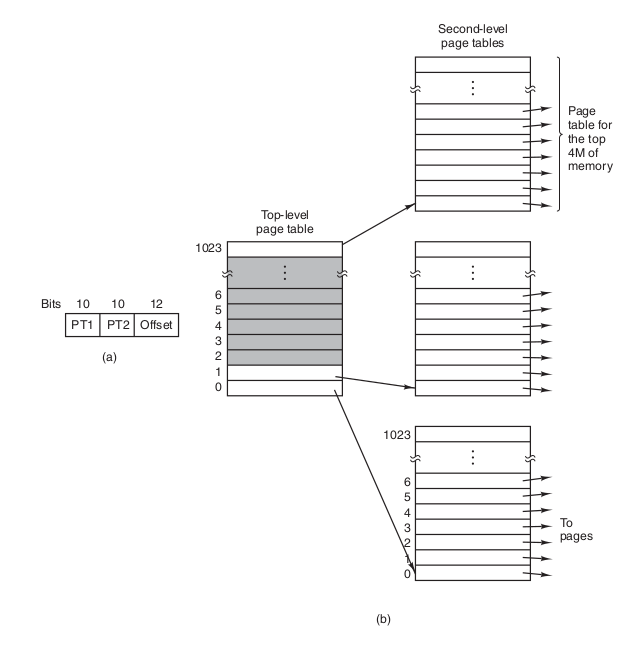
\includegraphics[width=0.5\textwidth]{imagenes/multilevel-page-table}
	\caption{Descomposición de una dirección virtual en paginación multinivel}
	\label{fig:multilevel-page-table}
\end{figure}

El directorio de páginas contiene información sobre como ubicar la tabla de páginas que necesitamos para mapear la dirección virtual. De esta forma, cuando la MMU recibe un dirección virtual, la divide en tres partes:

\begin{itemize}
	\item Los primeros bits son usados como índice para ubicar la entrada en el directorio de páginas que nos permite conseguir la tabla correspondiente a esa dirección.
	\item La segunda parte se usa como número de página dentro de esa tabla para encontrar el page frame deseado.
	\item Y la última parte es el offset dentro del page frame encontrado.
\end{itemize}

La entrada del directorio de páginas es igual que la de una tabla de páginas normal. Si el bit de presente no está activado cuando buscamos una tabla determinada, se genera un page faul y el sistema operativo debe cargar en memoria la tabla correspondiente.

\subsection{Algoritmos de reemplazo de páginas}
El mejor algoritmo de remplazo de páginas es imposible de implementar: Remplazar la página que menos se va a utilizar en el futuro.

\subsubsection{Not Recently Used (NRU)}
Como dijimos, las entradas de las tablas de páginas tienen dos bits (bit dirty y referenced) que nos dan información sobre como se estuvo usando cada una de ellas. Gracias a ellos, se pueden crear algoritmos de paginación con distintos criterios que nos permitan saber como remplazar page frames a medida que se van ejecutando los procesos.

Cuando un proceso comienza su ejecución, ambos bits están desactivados para todas las entradas de la tabla. Además, el bit de referencia se desactiva periódicamente para distinguir las entradas que fueron accedidas recientemente de aquellas que no.

Cuando ocurre un page fault, el sistema operativo inspecciona todas las páginas y las divide en 4 categorías:

\begin{itemize}
	\item Clase 0: No referenciadas, no modificadas
	\item Clase 1: No referenciadas, modificadas
	\item Clase 2: Referenciadas, no modificadas
	\item Clase 3: Referenciadas y modificadas
\end{itemize}

El algoritmo NRU remueve una página random de la clase más baja no vacía. En este algoritmo está implicita la ideae de que es mejor swapear una página modificad que hace rato que no se referencia, a una página no modificada que se está usando.

\subsubsection{First In, Firt Out (FIFO)}
El sistema operativo mantiene una lista de todas las páginas cargadas en memoria. La última página de esta lista es la ultima que fue cargada y la primer es la que más tiempo estuvo en memoria.

Cuando se realiza un page faul, se remueve el primer elemento y se encola la nueva página.

\paragraph{Second Chance Algorithm:} Se modifica el FIFO para que se inspecciones el bit de referencia de la página más vieja. Si el bit está en cero, entonces la página es vieja y no está en uso por lo que es remplazada. 

Si el bit está seteado, entonces el bit se limpia y la página se encola al final de la lista. Luego, la búsqueda continua. Si todas las páginas fueron referenciadas, entonces, se revisan todas las páginas cargadas hasta volver a empezar y se termina eliminando la que había sido la primer página analizada.

\subsubsection{Least Recently Used}
Una buena aproximación al algoritmo optimo se basa en la observación que las páginas que han sido más usadas en las últimas instrucciones probablemente vuelvan a ser usadas. En cambio, las páginas que no son usadas hace rato probablemente sigan sin usarse.

En este algoritmo, cuando sucede un page fault, se descarga la página que no ha sido usada durante el mayor rango de tiempo.

\subsubsection{Working Set}
En su forma más pura, los procesos comienzan sin ninguna de páginas en memoria. Tan pronto como el CPU trata de conseguir la primer instrucción se produce un page fault, causando que el sistema operativo traiga la página que contiene la primer instrucción. Por lo general, se producen varios page fault para traer memoria variables globales y el stack. 

Después de un tiempo, el proceso tiene la mayoría de las páginas que necesita para poder ejecutar con relativamente pocos page fault. Esta estrategia se llama \textbf{demand paging} porque ninguna página se carga a no ser que sea necesaria.

La mayoría de los procesos exhiben \textbf{localidad de referencia}, esto significa que durante cualquier etapa de ejecución el proceso referencia solo una pequeña fracción de sus páginas disponible. 

El conjunto de páginas que un proceso está usando se llama conjunto de trabajo (\textbf{working set}). Si este conjunto entra complentamente en memoria, entonces el proceso podrá correr realizando poco page faults. Si la memoria disponible no alcanza para almacenarlo entonces el proceso generara page faults constantemente y se alentizará su ejecución. Este efecto se llama \textbf{trashing}.

Por esta razón, muchos sistemas tratan hacer un seguimiento del working set de cada proceso y asegurarse que esté completamente en memoria antes de dejar que se ejecute. Este método se llama \textbf{working set model} y está diseñado para disminuir el ratio de page faults provocados por proceso. Cargar páginas antes de que los procesos la necesiten es una técnica llamada \textbf{prepaging}

\subsection{Page fault}
Estos son los pasos que realiza un sistema opertivo una vez que el MMU emite un page fault:

\begin{enumerate}
	\item El hardware emite el page fault que es atrapado por el sistema operativo.
	\item Se guarda el program counter de la instrucción fallida y el estado del proceso.
	\item El sistema operativo se fija cual es la página que necesita el proceso. 
	\item El sistema operativo controla que la dirección pedida sea válida y que la protección de la misma sea consistente con el acceso. Si no lo es, se manda una señal al proceso o se lo mata. Si la dirección es válida y no hay un protection fault, el sistema se fija si hay page frames libres. Si no los hay, se usa alguno de los algoritmos de remplazo de páginas.
	\item Si el page frame a desalojar está modificado, la página se marca para transferir a disco. Se realiza un context switch suspendiendo la rutina de interrupción y dejando que otro proceso se ejecute mientras se completa la transferencia.
	\item Una vez completada la transferencia, el sistema operativo, busca la dirección del disco en la que está almacenada la página y la marca para cargarla en memoria. Mientras sucede esta transferencia se vuelve a suspender la rutina y se deja ejecutar a otro proceso.
	\item Despues de que la página está cargada en memoria, se actualizan las tablas de página para reflejar los cambios y la entrada se marca como válida.
	\item El proceso vuelve a entrar en la cola del scheduler y el estado se reseta a como estaba antes de ejecutar la instrucción que generó el page fault.
\end{enumerate}

\printbibliography[keyword=memoriaVirtual, title=Bibliografía]

\newpage
\section{Segmentación}
La memoria virtual discutida hasta ahora es unidimensional: A cada proceso se le asigna un conjunto de direcciones que van desde 0 hasta una dirección máxima. Cuando el compilador genera un proceso divide este espacio en partes de uso espécifico (por ejemplo, stack, tabla de constantes, tabla de símbolos, código fuente, etc). 

Sin embargo, esta division puede llegar a traer problemas. En la figura \ref{fig:organizacion-proceso}, por ejemplo,  la tabla de símbolos se llenó y no puede seguir creciendo porque las próximas direcciones contienen el código del programa.

\begin{figure}[h]
	\centering
	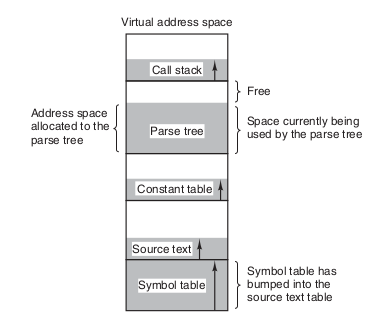
\includegraphics[width=0.7\textwidth]{imagenes/organizacion-proceso-virtual-unidimensional}
	\caption{Organización de un proceso con memoria virtual }
	\label{fig:organizacion-proceso-virtual-unidimensional}
\end{figure}

Una solución a este problema es proveer al proceso de varios espacios de memoria virtuales completamente independientes llamados \textbf{segmentos}. Cada segmentos consiste en una secuencia lineal de direcciones que van desde cero hasta algún valor máximo y como son independiente cada uno puede crecer o contraer sin afectarse entre si.

Para especificar una dirección ubicada en un segmento, el programa debe enviar una dirección que se divide en dos partes: Un número de segmento y la dirección virtual dentro de ese segmento.

Esta técnica además facilita la implementación de librerias compartidas. Dado que cada fragmento es una entidad lógica que el programador sabe que contiene, cada uno de ellos puede tener distinto tipos de protección.

En muchos sitemas es común encontrar la segmentación implementada con paginación para segmento.

\subsection{Shared Libraries}
En sistemas multiprogramables, es comun tener varios usuarios corriendo el mismo programa de manera simultánea. Incluso un único usuario puede estar corriendo varios programas que hagan uso de las mismas rutinas. Cuando esto sucede, los segmentos de código de cada proceso apuntan a la misma tabla de páginas (como el código es solo lectura, ambos procesos pueden accederlas sin problemas).

Sin embargo, hay que tener en cuenta que cuando dos o mas procesos comparten las páginas y uno termina, no debemos desalojar las páginas compartidas ya que cuando se vuelva a ejecutar el otro proceso, se generarian varios page faults hasta que todas las paǵinas desalojadas vuelvan a estar en memoria. Por esta razón, debemos mantener una estructura que nos permita identificar rápidamente cuales son las páginas compartidas para evitar esta situación.

\subsubsection{Copy On Write}
Tambien se puede compartir páginas que contenga datos aunque hay que tener algunas consideraciones más. En los sistemas UNIX, en particular, cuando se realiza una llamada a \texttt{fork()}, el proceso padre comparte todas sus páginas con el proceso hijo pero cada uno tiene su propio conjunto de tablas de páginas. Sin embargo, en ambos procesos se marca a todas las páginas como \textit{Read Only}. 

Mientras ambos procesos solo hagan lecturas, la situación se mantiene. Tan pronto como algunos de los dos necesita realizar una modificación, se genera un protection fault que es interceptado por el sistema operativo. El mismo realiza una copia de la página que se quiere modificar y ahora cada proceso tiene su propia copia de la información con acceso de escritura/lectura. Así, las próximas modificaciones a esa página suceden sin interrupciones. Esto implica que la información que las páginas que no son modificadas nunca no necesitan ser copiadas.

Esta técnica es conocida como \textbf{copy on write}.

\printbibliography[keyword=segmentacion, title=Bibliografía]
 
 